\documentclass[10pt,twocolumn]{article}

\IfFileExists{neurips_2024.sty}{
  \usepackage[final]{neurips_2024}
}{
  \usepackage[margin=0.8in]{geometry}
  \usepackage{titlesec}
  \setlength{\columnsep}{0.25in}
}

\usepackage[T1]{fontenc}
\usepackage[utf8]{inputenc}
\usepackage{lmodern}
\usepackage{microtype}
\usepackage{amsmath, amssymb}
\usepackage{booktabs}
\usepackage{multirow}
\usepackage{graphicx}
\usepackage{caption}
\usepackage{subcaption}
\usepackage{array}
\usepackage{tabularx}
\usepackage{enumitem}
\usepackage{xcolor}
\usepackage{hyperref}
\hypersetup{colorlinks=true, citecolor=blue, linkcolor=blue, urlcolor=blue}

\title{Sparse Signal-Field SAEs for Hierarchical Vision Representations}
\author{Jason Peng}
\date{June 2026}

\begin{document}
\maketitle

\begin{abstract}
We study whether intermediate vision activations are sparse in a learned transform domain and whether those sparse codes form a stable hierarchy across depth. Using frozen ResNet backbones on CIFAR-100 and CIFAR-10, we train sparse autoencoders (SAEs) on activation fields at five depths and retain only a small fraction of learned feature-location coefficients. A convolutional Field SAE preserves downstream classification at 2--5\% retained coefficients across all sections, materially outperforming both a pointwise Vector SAE and linear or random-code baselines. We then test whether sparse codes at one depth predict sparse codes at the next. Single-step transitions are strong, and a frozen-block hybrid chain shows that the sparse support is information-sufficient end-to-end. Naive learned multi-step chaining initially collapses, but re-grounding, scheduled-sampling, and later rollout-aligned retraining recover most of the gap to the causal upper bound. Follow-up runs strengthen the story with seed stability, transfer to ResNet-110 and ResNet-20/CIFAR-10, sparse-vs-dense transition taxonomy, causal intervention evidence, and a first ViT transfer artifact. The resulting picture is that learned sparse field codes are both behavior-preserving and structurally meaningful, while stable hierarchical rollout depends on matching training and evaluation to the sparse-code manifold.
\end{abstract}

\section{Introduction}
Sparse autoencoders have become a useful way to probe learned representations, but most SAE work treats activations as vectors. Convolutional vision backbones instead expose activation fields with explicit spatial structure, so a sparse representation should preserve both \emph{what} feature is active and \emph{where} it is active. This project asks two questions:
\begin{enumerate}[leftmargin=1.2em]
  \item Can a CNN activation field be reconstructed from a very sparse set of learned feature-location coefficients without changing the network's prediction?
  \item Do sparse codes at one depth generate sparse codes at the next, forming a depth-wise sparsity tree?
\end{enumerate}

Our core setting is a frozen ResNet-56 on CIFAR-100 with baseline top-1 accuracy of 71.83\%. We tap five sections ($Q1\dots Q5$), train SAEs independently at each section, and evaluate reconstructions by splicing them back into the frozen model and measuring the resulting classifier behavior. We then learn section-to-section transitions in sparse-code space and compare them against a frozen-block hybrid upper bound that uses the real backbone blocks between sparse codes.

The main contributions are:
\begin{itemize}[leftmargin=1.2em]
  \item A convolutional \emph{Field SAE} that learns sparse codes over feature-location fields and strongly outperforms a pointwise \emph{Vector SAE} at aggressive budgets.
  \item Evidence that 2--5\% retained sparse coefficients are sufficient to preserve near-original behavior across five CNN depths.
  \item A hierarchy study showing that sparse support is causally sufficient end-to-end, while stable learned chaining requires re-grounding or rollout-aligned training.
  \item Follow-up robustness and transfer results spanning seed stability, new backbones, sparse-vs-dense transition comparison, causal interventions, and an initial ViT artifact.
\end{itemize}

\section{Method}
\subsection{Backbone, sections, and evaluation}
We use a frozen ResNet-56 trained on CIFAR-100 and evaluate five post-activation sections:
\begin{center}
\small
\begin{tabular}{lcc}
\toprule
Section & Shape & Description \\
\midrule
$Q1$ & $16 \times 32 \times 32$ & post-stem \\
$Q2$ & $16 \times 32 \times 32$ & end of stage 1 \\
$Q3$ & $32 \times 16 \times 16$ & end of stage 2 \\
$Q4$ & $64 \times 8 \times 8$ & mid stage 3 \\
$Q5$ & $64 \times 8 \times 8$ & end of stage 3 \\
\bottomrule
\end{tabular}
\end{center}

For each section we cache activations and train an SAE with overcomplete width $K = 8C$. Given activation field $H \in \mathbb{R}^{C \times H \times W}$, the SAE produces a code field $Z \in \mathbb{R}^{K \times H \times W}$, applies a hard TopK mask $\tilde{Z}$, and reconstructs $\hat{H}$. Reconstruction quality is measured by relative $\ell_2$, cosine similarity, and most importantly \emph{spliced top-1}: replace the true activation with $\hat{H}$, run the frozen tail, and compare classifier outputs to the original network.

\subsection{SAE architectures and masks}
We compare two SAE families:
\begin{itemize}[leftmargin=1.2em]
  \item \textbf{Vector SAE:} a shared pointwise encoder/decoder applied independently at each spatial location.
  \item \textbf{Field SAE:} a convolutional encoder/decoder with local residual blocks and depthwise spatial mixing before the sparse bottleneck.
\end{itemize}

We also compare two masking schemes:
\begin{itemize}[leftmargin=1.2em]
  \item \textbf{Global mask:} retain the top fraction of coefficients over the whole field.
  \item \textbf{RF-local mask:} retain top coefficients within receptive-field windows of the next section.
\end{itemize}

SAEs are trained with a staged curriculum: warmup without sparsity, annealing from 50\% retained to the target budget, then fixed-budget training. This curriculum substantially stabilizes learning relative to a cold start at the final sparsity level.

\subsection{Hierarchy experiments}
For the winner SAE configuration we learn adjacent transitions $T_t: \tilde{Z}_t \rightarrow \hat{Z}_{t+1}$ and evaluate:
\begin{itemize}[leftmargin=1.2em]
  \item \textbf{Single-step learned transitions:} sparse code at $Q_t$ predicts sparse code at $Q_{t+1}$.
  \item \textbf{Frozen-block hybrid chain:} decode sparse code, run the real frozen backbone block, then re-encode; this isolates whether the sparse support contains enough information independent of predictor error.
  \item \textbf{Multi-step learned chaining:} compose all learned transitions from $Q1$ to $Q5$, optionally with re-masking or re-grounding.
\end{itemize}

Re-grounding means decode $\rightarrow$ re-encode $\rightarrow$ re-mask after each predicted step, projecting the rollout back onto the SAE manifold.

\section{Sparse Reconstruction Results}
Phase 1 establishes the anchor result: sparse reconstruction is enough to preserve downstream behavior.

\begin{figure}[t]
  \centering
  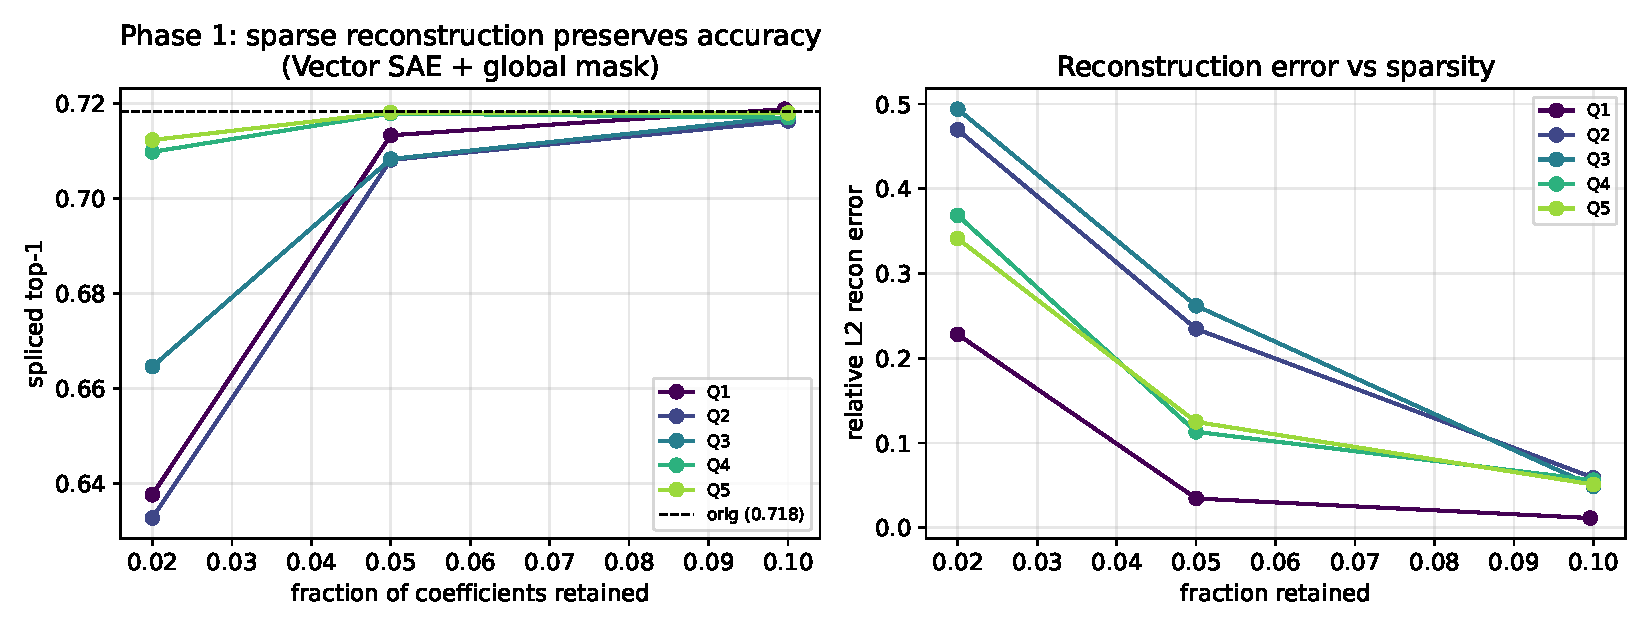
\includegraphics[width=\columnwidth]{figures_pdf/fig1_phase1_curves.pdf}
  \caption{Phase 1 reconstruction curves. Spliced accuracy stays near the original classifier performance at small retained fractions, especially in deeper sections.}
  \label{fig:phase1}
\end{figure}

\begin{table}[t]
\centering
\small
\caption{Representative Vector SAE + global-mask results from Phase 1.}
\label{tab:phase1}
\begin{tabular}{lcccc}
\toprule
Section & Fraction & RelL2 & Cos & Top-1 \\
\midrule
Q1 & 5\% & 0.034 & 0.999 & 0.713 \\
Q2 & 10\% & 0.059 & 0.998 & 0.716 \\
Q3 & 10\% & 0.049 & 0.999 & 0.717 \\
Q4 & 2\% & 0.369 & 0.929 & 0.710 \\
Q5 & 2\% & 0.341 & 0.939 & 0.712 \\
\bottomrule
\end{tabular}
\end{table}

Table~\ref{tab:phase1} and Figure~\ref{fig:phase1} show that every section reaches near-original top-1 accuracy with only 2--10\% of coefficients retained, and deeper sections preserve accuracy even at 2\%. The result is not trivial autoencoding: a random-dictionary control is near chance, while a matched-budget PCA baseline is consistently weaker.

\begin{figure}[t]
  \centering
  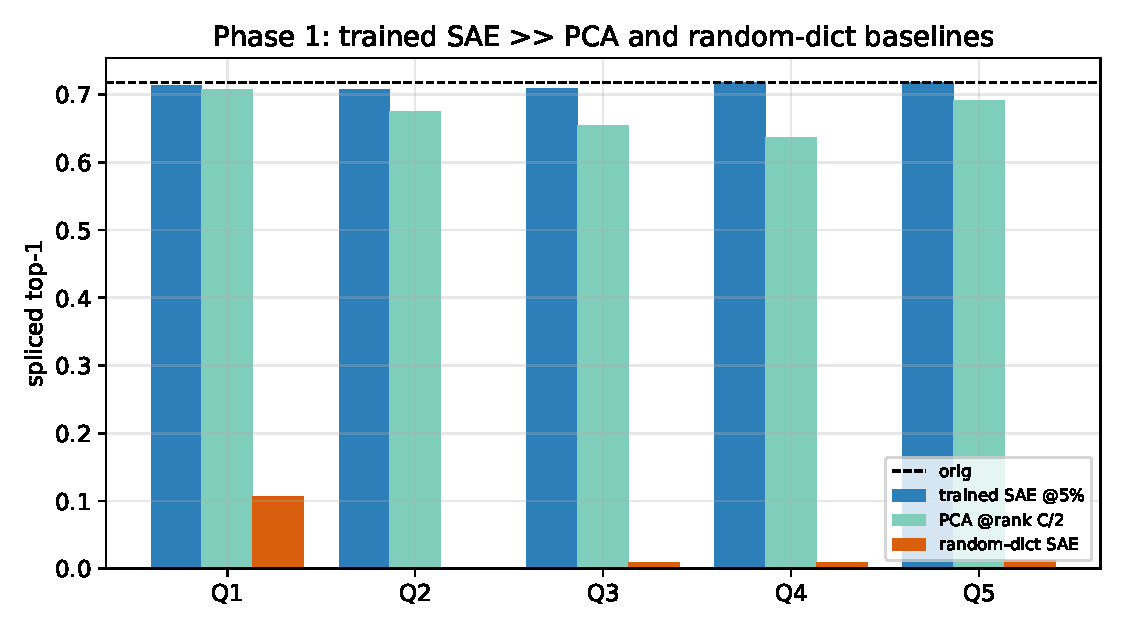
\includegraphics[width=\columnwidth]{figures_pdf/fig2_baselines.pdf}
  \caption{The trained SAE strongly outperforms PCA and a random-dictionary control. Sparse reconstruction quality is therefore learned rather than a budget artifact.}
  \label{fig:baselines}
\end{figure}

This confirms the transform-domain sparsity hypothesis for the anchor backbone: hidden fields may look dense in pixel-channel coordinates, yet they are highly compressible in a learned sparse basis.

\section{Architecture and Masking Choices}
Phase 2 compares the SAE architecture and mask type. The central result is that the convolutional Field SAE materially outperforms the pointwise Vector SAE at aggressive budgets, especially in early high-resolution sections.

\begin{figure}[t]
  \centering
  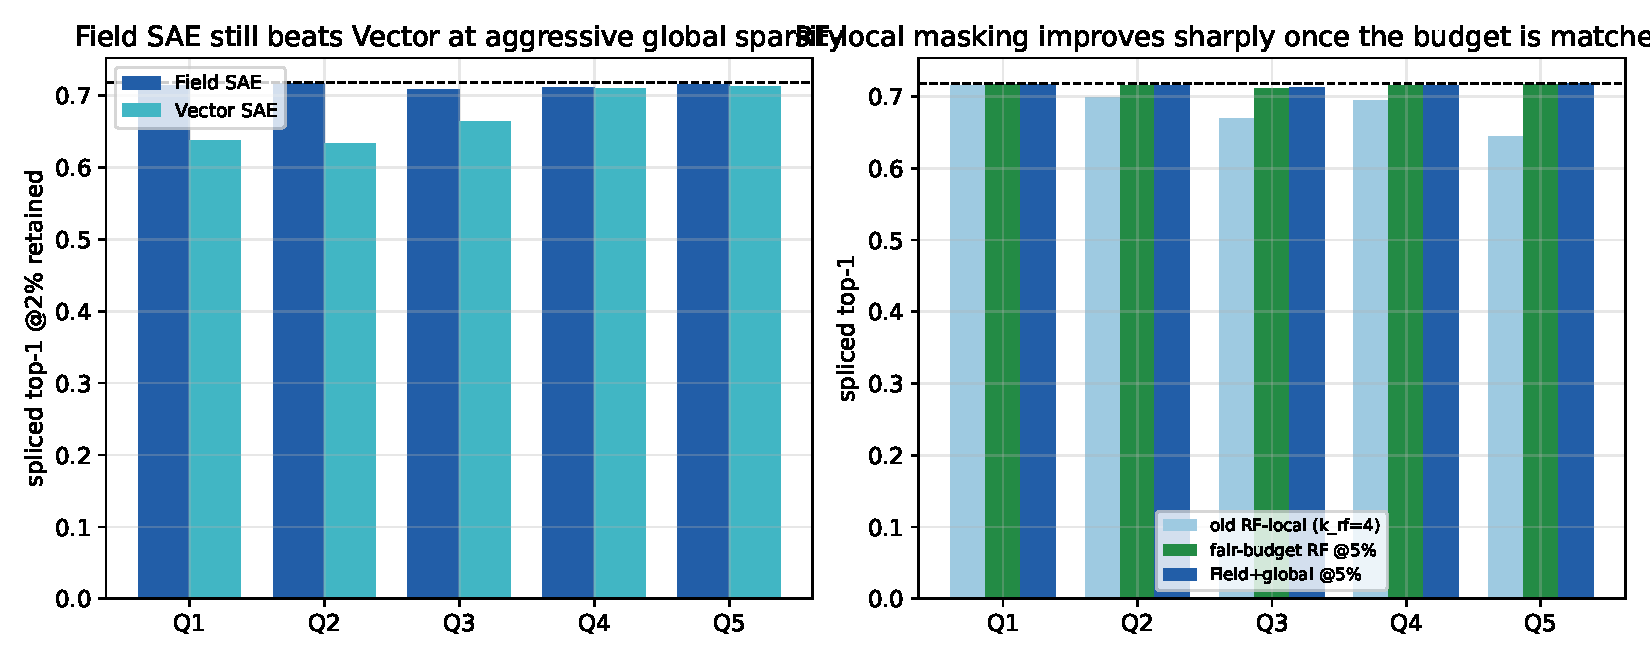
\includegraphics[width=\columnwidth]{figures_pdf/fig3_field_vs_vector.pdf}
  \caption{Field SAE versus Vector SAE. Local spatial mixing is especially valuable in early sections at low retained fractions.}
  \label{fig:field-vs-vector}
\end{figure}

\begin{table}[t]
\centering
\small
\caption{Spliced top-1 at 2\% retained with global masking.}
\label{tab:field-vector}
\begin{tabular}{lccc}
\toprule
Section & Field & Vector & Gain \\
\midrule
Q1 & 0.714 & 0.638 & +7.6 pp \\
Q2 & 0.716 & 0.633 & +8.3 pp \\
Q3 & 0.708 & 0.665 & +4.3 pp \\
Q4 & 0.711 & 0.710 & +0.1 pp \\
Q5 & 0.715 & 0.712 & +0.3 pp \\
\bottomrule
\end{tabular}
\end{table}

The Field SAE winner path is therefore the main basis for later hierarchy experiments. The original RF-local masking story looked much weaker, but a later fair-budget rerun revised that interpretation: once RF budgets are normalized fairly per window, RF-local masking becomes competitive with the global path rather than fundamentally broken.

\section{Sparse-Code Hierarchy}
\subsection{Single-step transitions}
Adjacent sparse-code transitions are generally strong, especially on easier edges.

\begin{figure}[t]
  \centering
  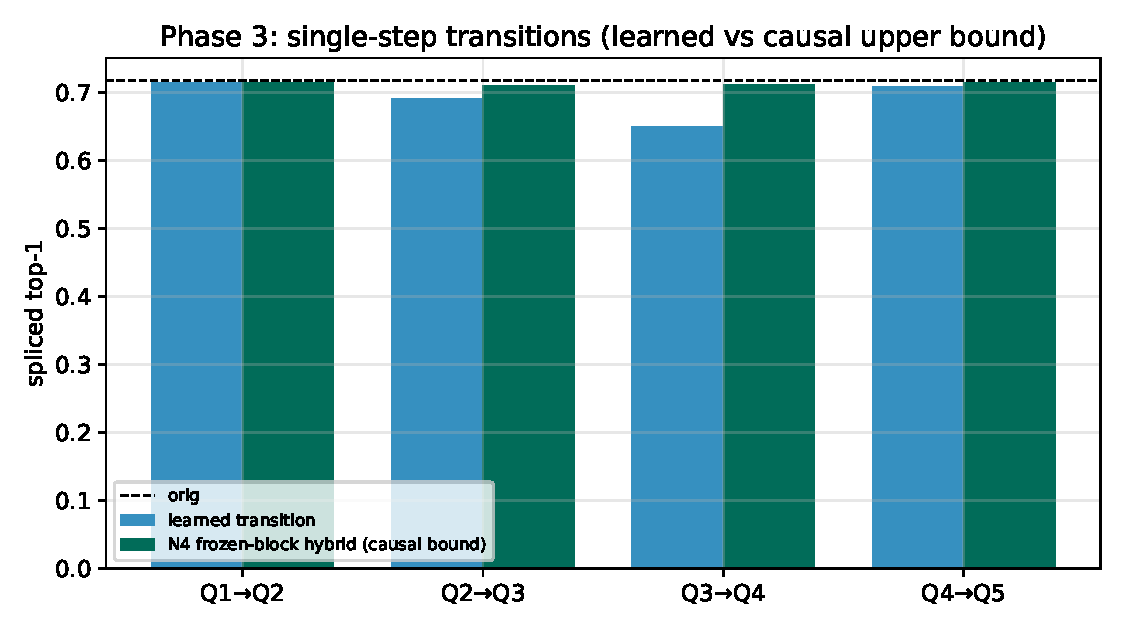
\includegraphics[width=\columnwidth]{figures_pdf/fig4_transitions.pdf}
  \caption{Single-step transition results. The learned $Q1 \rightarrow Q2$ transition matches the frozen-block hybrid upper bound, while $Q3 \rightarrow Q4$ is the consistent bottleneck.}
  \label{fig:transitions}
\end{figure}

\begin{table}[t]
\centering
\small
\caption{Single-step transition accuracy versus the frozen-block hybrid upper bound.}
\label{tab:transitions}
\begin{tabular}{lcc}
\toprule
Transition & Learned & Hybrid \\
\midrule
Q1 $\rightarrow$ Q2 & 0.715 & 0.715 \\
Q2 $\rightarrow$ Q3 & 0.691 & 0.711 \\
Q3 $\rightarrow$ Q4 & 0.650 & 0.711 \\
Q4 $\rightarrow$ Q5 & 0.709 & 0.715 \\
\bottomrule
\end{tabular}
\end{table}

The learned predictor exactly matches the hybrid bound on $Q1 \rightarrow Q2$, while $Q3 \rightarrow Q4$ remains the hardest step throughout the project. That persistent bottleneck later reappears in both ResNet-110 and taxonomy follow-ups, suggesting that it reflects a genuine representational difficulty rather than simple noise.

\subsection{Multi-step chaining}
The first raw learned chain collapses under recursive rollout even though the hybrid chain preserves near-original accuracy. This separation is crucial: the sparse support contains enough information, but naive sparse-code prediction suffers from exposure bias and manifold drift.

\begin{figure}[t]
  \centering
  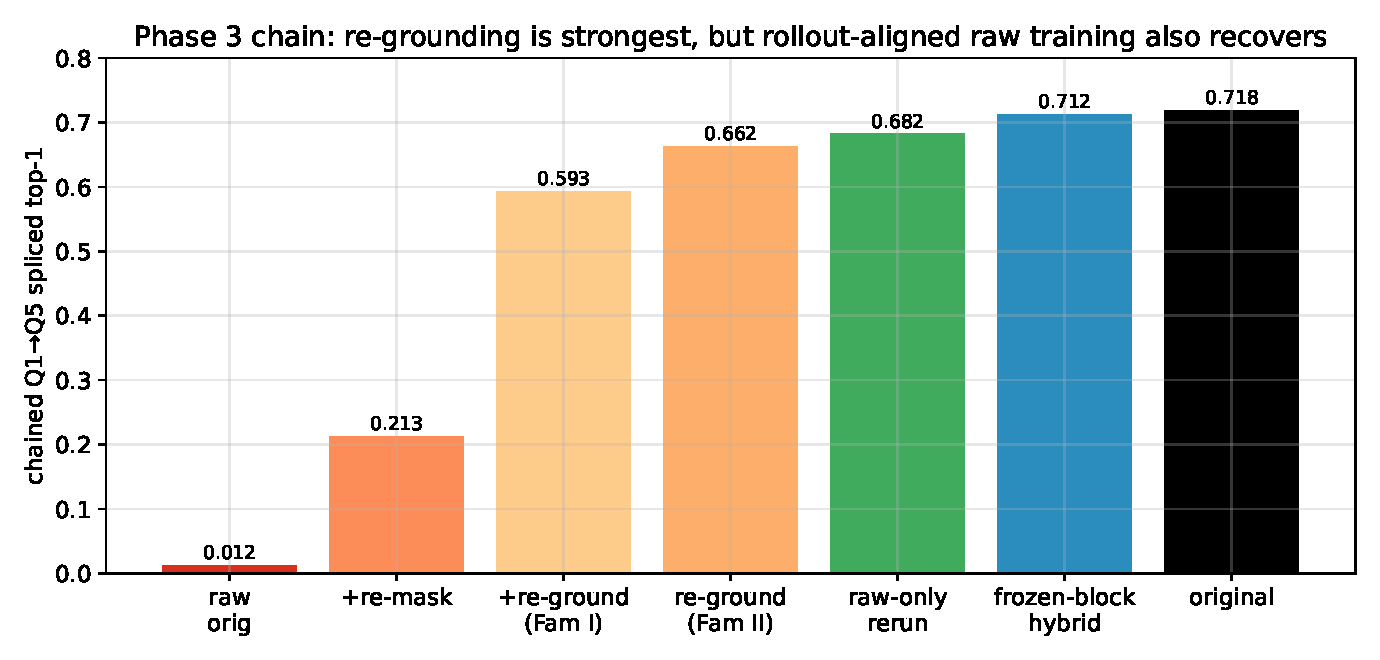
\includegraphics[width=\columnwidth]{figures_pdf/fig5_chain.pdf}
  \caption{Chained rollout variants. The hybrid chain nearly preserves original accuracy, while naive raw chaining collapses and re-grounding recovers much of the gap.}
  \label{fig:chain}
\end{figure}

\begin{figure}[t]
  \centering
  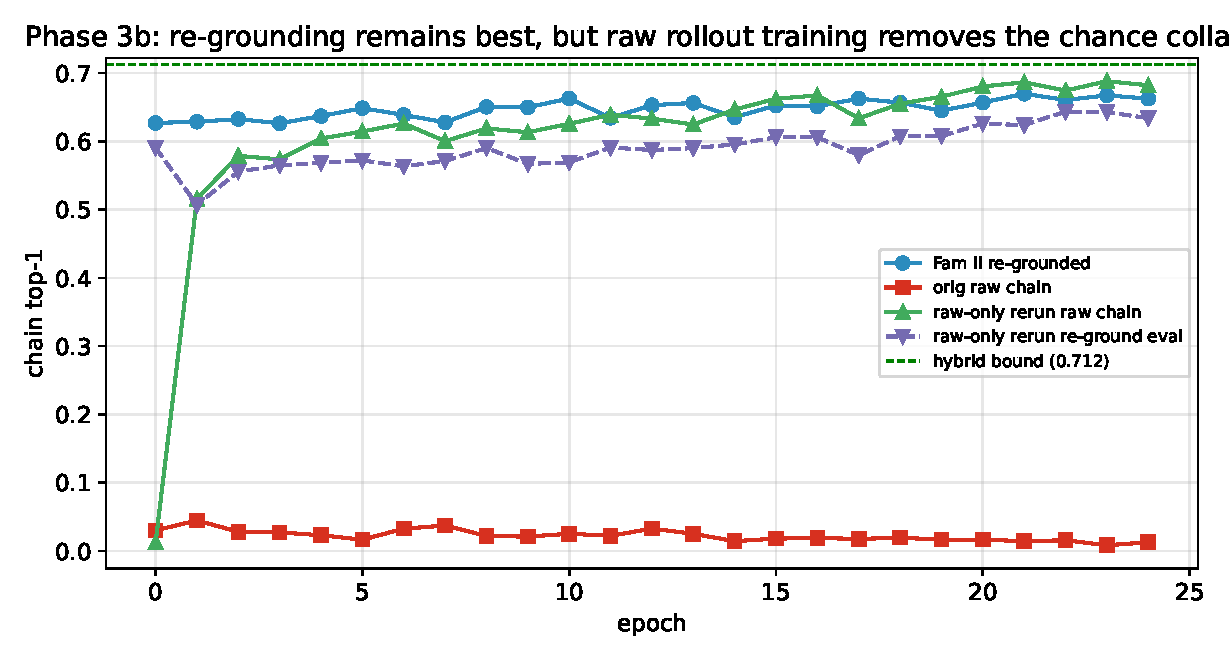
\includegraphics[width=\columnwidth]{figures_pdf/fig6_phase3b.pdf}
  \caption{Chain-aware training improves the re-grounded learned chain from 0.593 to 0.662, narrowing the gap to the 0.712 causal upper bound.}
  \label{fig:phase3b}
\end{figure}

\begin{table}[t]
\centering
\small
\caption{End-to-end chain accuracy from $Q1$ to $Q5$.}
\label{tab:chain}
\begin{tabular}{lc}
\toprule
Variant & Top-1 \\
\midrule
Raw learned chain & 0.012 \\
Re-mask each step & 0.213 \\
Re-ground each step & 0.593 \\
Scheduled-sampling + re-ground & 0.662 \\
BPTT through re-grounding & 0.701 \\
Frozen-block hybrid chain & 0.712 \\
Original classifier & 0.718 \\
\bottomrule
\end{tabular}
\end{table}

At first glance, these results suggested that re-grounding was strictly necessary. Later changed reruns refined that conclusion. A rollout-aligned \emph{raw-only} retraining run, with scheduled sampling, full-chain BPTT, and gradient clipping but without re-grounding on the carrier path, recovers a strong raw chain at 0.682. This means the original collapse was partly an exposure-bias problem rather than proof that raw sparse-code chaining is impossible. Re-grounding remains the cleanest and strongest stabilization mechanism in the artifact record, but it is no longer the only viable one.

\section{Intervention, Sparsity, and Worked Examples}
Beyond top-line accuracy, the project also asks whether the sparse codes are meaningful and structured.

\begin{figure}[t]
  \centering
  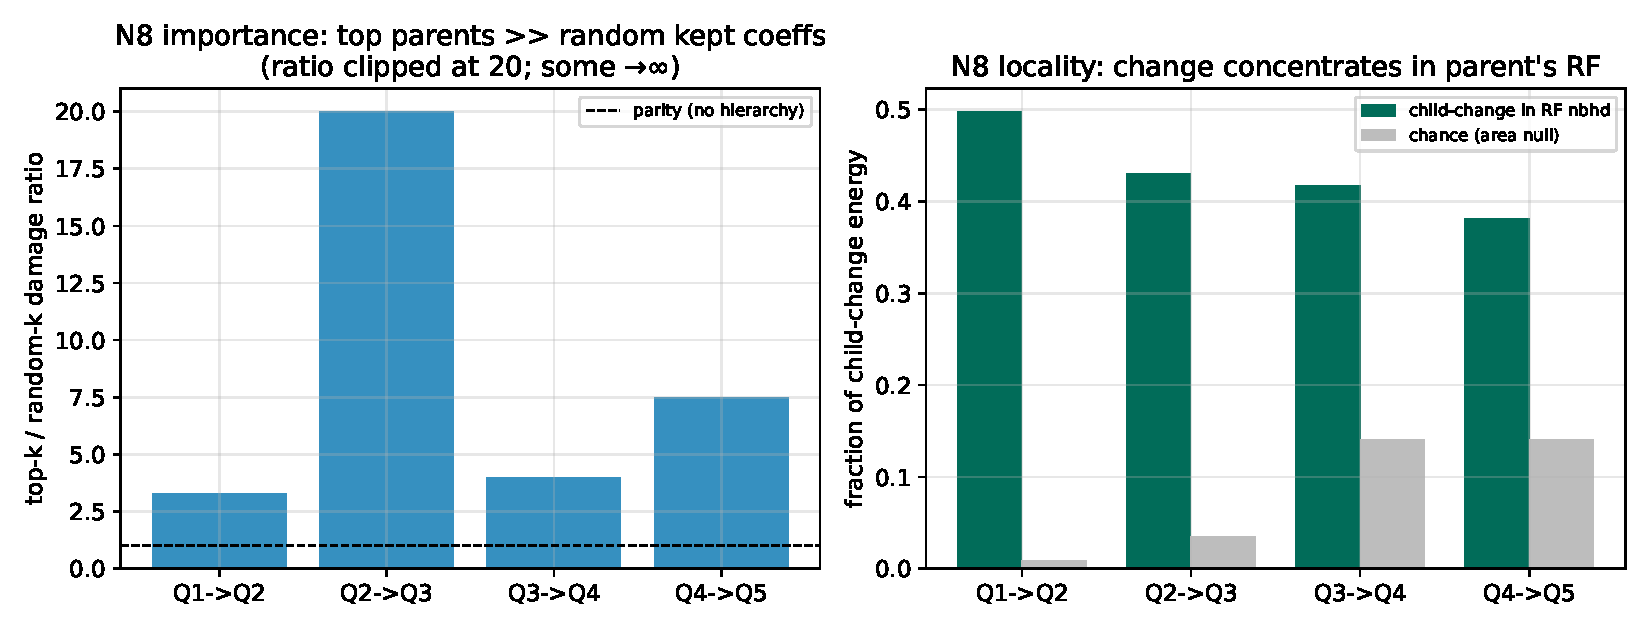
\includegraphics[width=\columnwidth]{figures_pdf/fig7_intervention.pdf}
  \caption{Parent-to-child intervention evidence. Ablating high-importance parent coefficients causes much larger downstream damage than random ablation, and changes concentrate locally in receptive-field neighborhoods.}
  \label{fig:intervention}
\end{figure}

\begin{figure}[t]
  \centering
  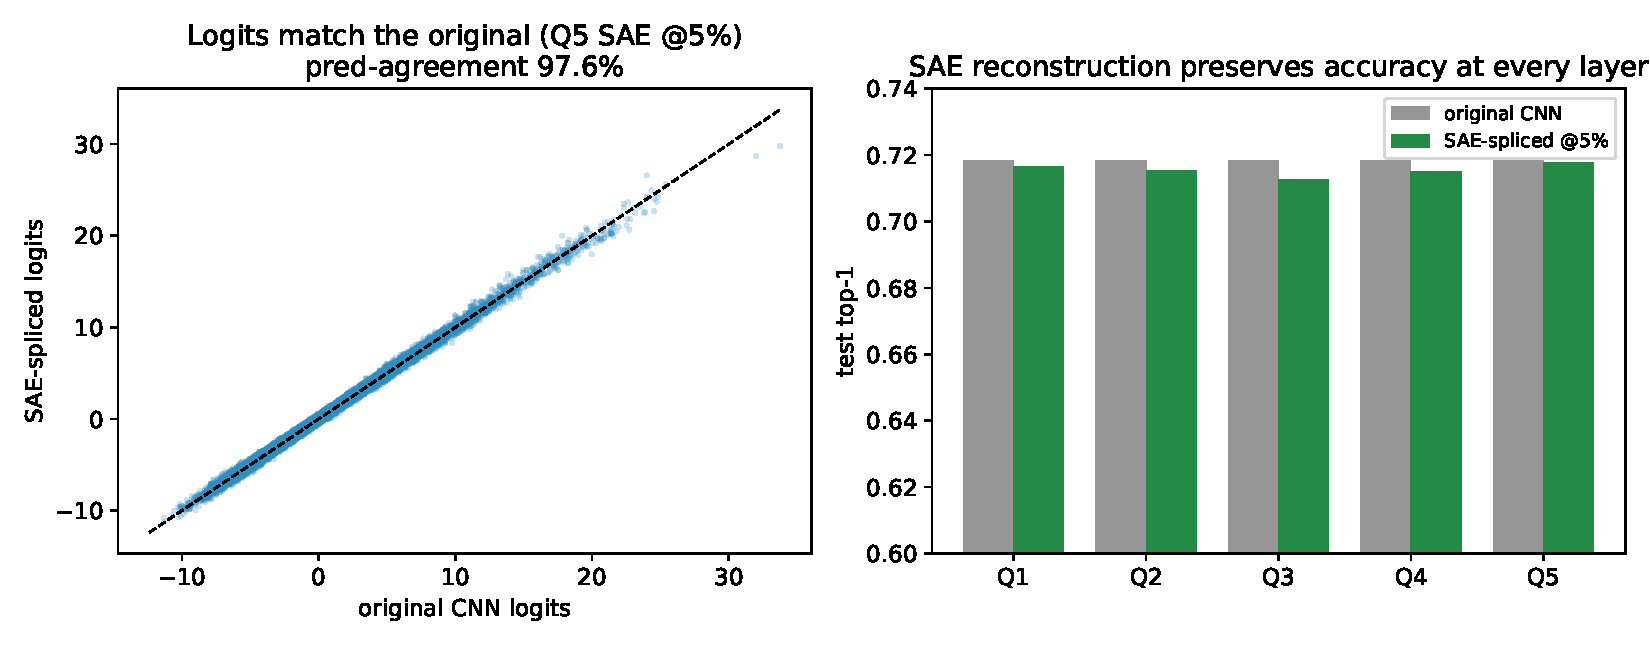
\includegraphics[width=\columnwidth]{figures_pdf/fig10_sae_vs_cnn.pdf}
  \caption{Worked comparison between SAE-spliced and original CNN behavior. Predictions agree on 97.6\% of test examples in the shown setting.}
  \label{fig:sae-vs-cnn}
\end{figure}

\begin{figure}[t]
  \centering
  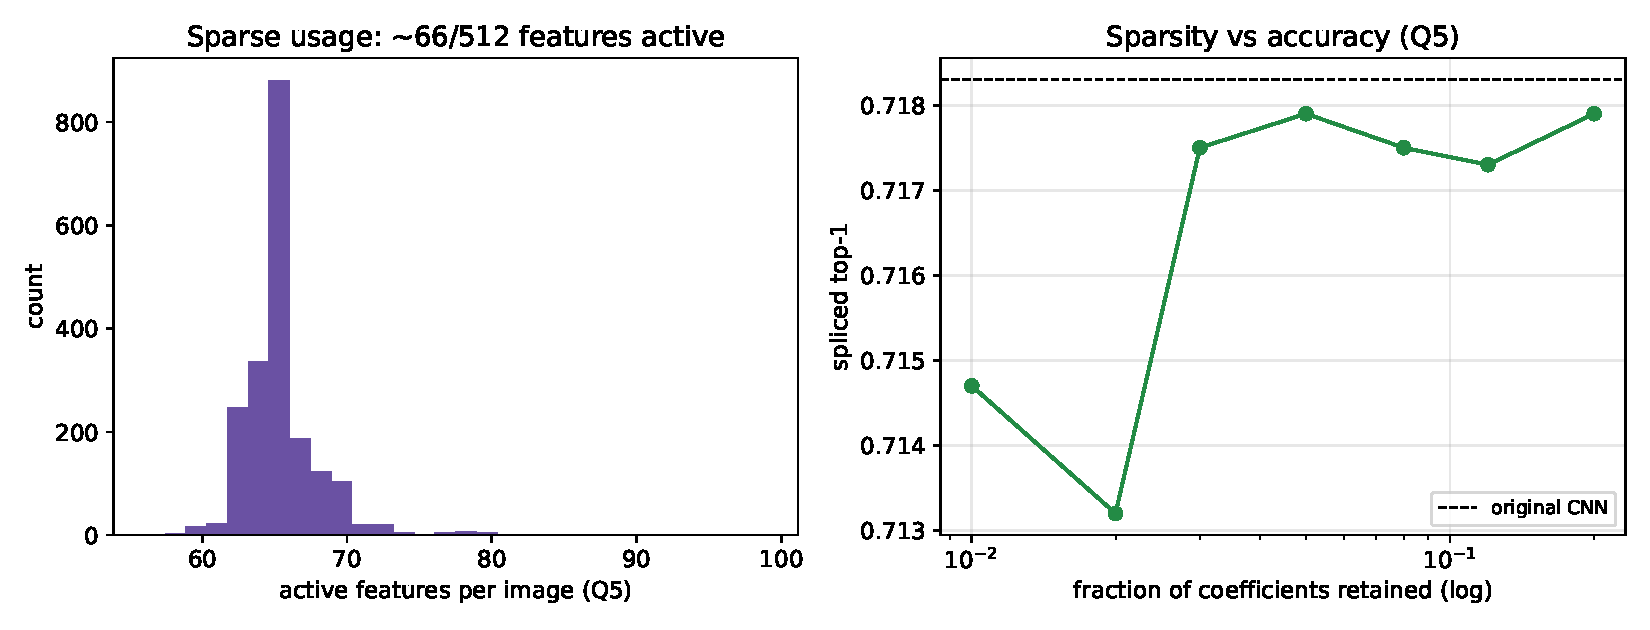
\includegraphics[width=\columnwidth]{figures_pdf/fig13_sparsity.pdf}
  \caption{Explicit sparsity diagnostics. Accuracy stays nearly flat down to a small retained fraction, then degrades sharply once the budget becomes too small.}
  \label{fig:sparsity}
\end{figure}

Intervention runs show that removing top-magnitude parent coefficients damages downstream behavior 3.3--7.5$\times$ more than ablating random kept coefficients, and 38--50\% of child-code change concentrates in the parent's receptive-field neighborhood. These results upgrade the hierarchy claim from purely predictive to causal and spatially directed. Feature audits additionally show low dead-feature and duplicate rates, indicating that the learned dictionaries are healthy rather than collapsed.

\section{Robustness and Transfer}
Phase 4 asks whether the winner-path story survives scale, seed variation, architecture shift, and a first transformer transfer.

\begin{table}[t]
\centering
\small
\caption{Selected Phase 4 extension results.}
\label{tab:phase4}
\begin{tabularx}{\columnwidth}{@{}lX@{}}
\toprule
Experiment & Main finding \\
\midrule
ResNet-20 / CIFAR-10 & All 15 cells succeed; deeper sections saturate near 92.3\% by 5\% retained. \\
Seed stability & Three seeds on ResNet-56/CIFAR-100 remain tightly clustered; means span 0.713--0.718. \\
Transition taxonomy & Sparse is the best $Q4 \rightarrow Q5$ carrier: 0.706 vs 0.690 dense and 0.610 cross. \\
ResNet-110 & The 5\% Field SAE preserves 0.723--0.732 top-1 across sections. \\
ViT transfer & At block 6 and 5\% retained, prediction agreement is 94.4\% with KL 0.043. \\
\bottomrule
\end{tabularx}
\end{table}

\begin{figure}[t]
  \centering
  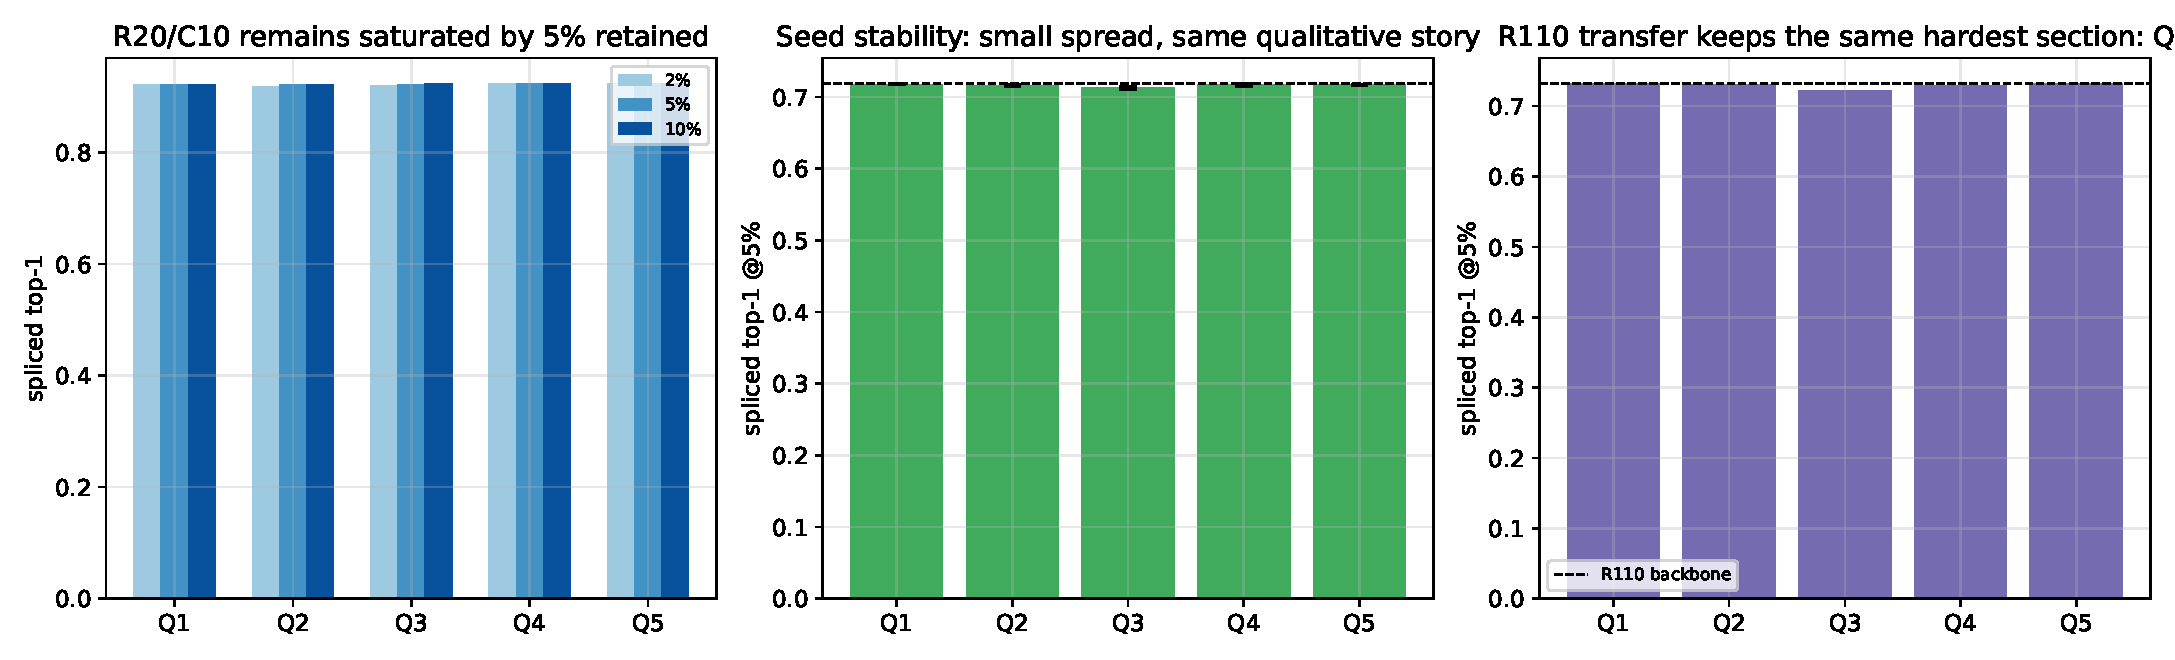
\includegraphics[width=\columnwidth]{figures_pdf/fig15_phase4_robustness.pdf}
  \caption{Phase 4 robustness summary. Winner-path behavior remains stable under seed variation and on a new ResNet-20/CIFAR-10 setting.}
  \label{fig:phase4-robustness}
\end{figure}

\begin{figure}[t]
  \centering
  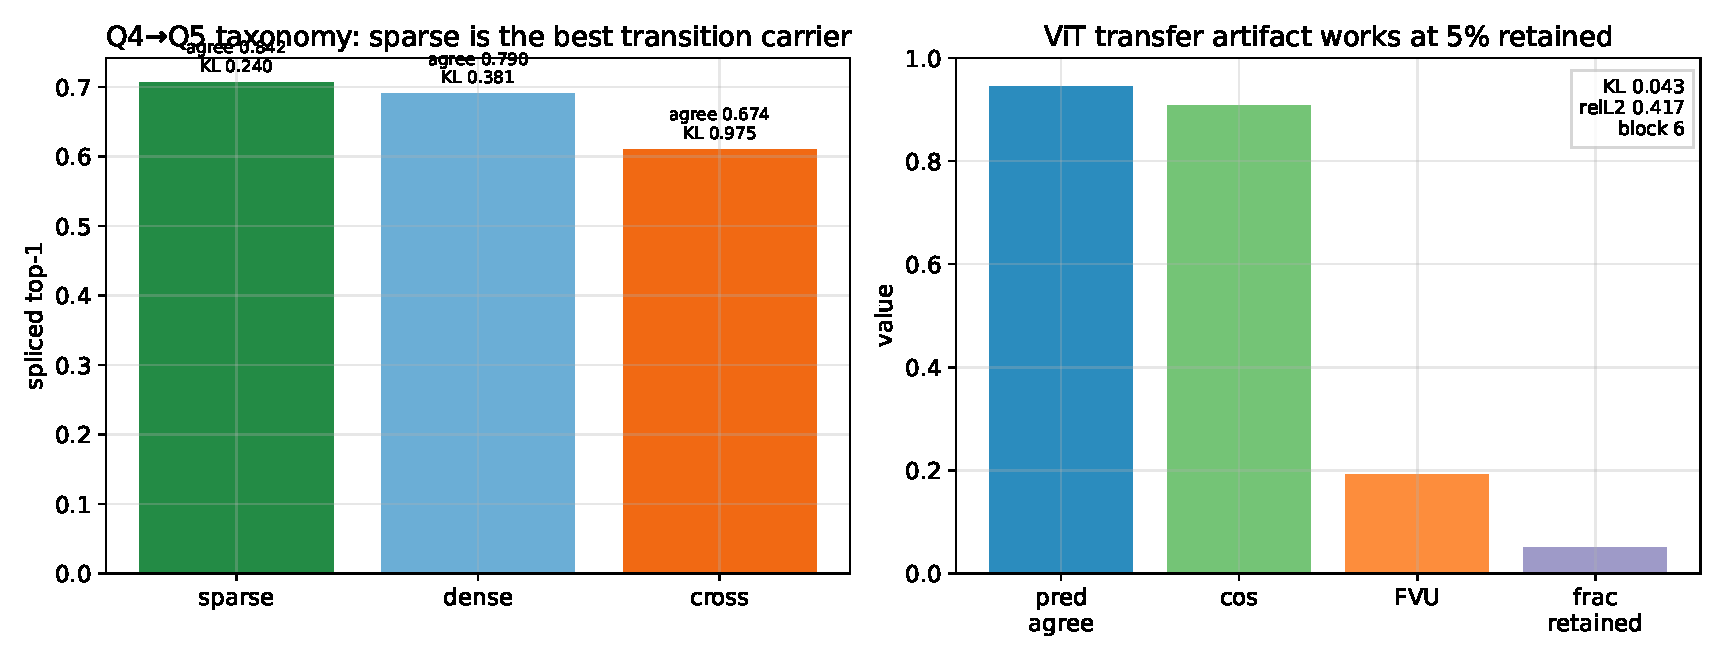
\includegraphics[width=\columnwidth]{figures_pdf/fig16_phase4_transfer.pdf}
  \caption{Phase 4 transfer summary. Sparse reconstruction extends to deeper CNNs and yields a first working ViT artifact.}
  \label{fig:phase4-transfer}
\end{figure}

These follow-ups materially strengthen the paper's empirical position. The winner-path conclusions are not single-seed accidents, not specific to one CNN depth profile, and not obviously tied to only one architecture family. The transition taxonomy result is especially important: sparse is not merely a reconstructive shortcut, but also the most behavior-preserving transition carrier among the tested alternatives.

\section{Limitations}
The project also has clear boundaries:
\begin{itemize}[leftmargin=1.2em]
  \item The development center of gravity is still one main anchor setting: ResNet-56 on CIFAR-100.
  \item The original Family II matrix breadth was not completed, even though chain-aware training on the winner path is substantial.
  \item The Q3 $\rightarrow$ Q4 transition remains the hardest step and is not fully solved by scaling predictor capacity alone.
  \item Patchwise changed reruns are informative but partially incomplete, especially for the depth-aware sweep.
  \item The ViT result is currently a strong transfer artifact rather than a full task-accuracy paper story.
\end{itemize}

These limitations narrow the strongest defensible claim: sparse field codes are clearly sufficient and behavior-preserving on the executed winner paths, and hierarchical rollout is real but sensitive to training distribution and manifold consistency.

\section{Conclusion}
The overall empirical picture is coherent. CNN activation fields are highly compressible in a learned sparse transform domain, and a convolutional Field SAE preserves classifier behavior while retaining only 2--5\% of feature-location coefficients. Sparse codes also carry real hierarchical information: they support strong one-step prediction, and their support is causally sufficient to drive the true network almost end-to-end at original performance. The main challenge is not whether sparse hierarchy exists, but how to train learned chains so that rollout stays on-manifold. Re-grounding, chain-aware training, and rollout-aligned retraining all help, with the best learned chain reaching 0.701 against a 0.712 hybrid upper bound and a 0.718 original baseline.

Taken together, the results support a practical and scientific claim: vision backbones compute with a sparse, spatially structured intermediate representation that can be compressed, propagated, and probed without destroying behavior. That makes sparse field codes a promising substrate for future mechanistic work, especially causal parent-child interventions, improved handling of the Q3 $\rightarrow$ Q4 bottleneck, and broader extension to transformer architectures.

\end{document}
